% slides.tex — the slide deck for the Physics of Deep Learning worksheet.
%
% Three lectures, stacked into one beamer document: Part I (Bayesian learning
% and phase transitions), Part II (networks at large width), Part III (neural
% scaling laws). They were written for the September 2026 Iliad Intensive and
% follow Sections 2, 3--5 and 7 of main.tex; the one-day teaching plan in
% Section 0 of main.tex says how they were used. Any self-contained LaTeX works
% here: the build compiles this file to slides.pdf and hosts it beside the
% worksheet's downloads (never converted to MDX).
\documentclass[11pt]{beamer}

\usetheme{default}
\usecolortheme{seahorse}
\setbeamertemplate{navigation symbols}{}
\setbeamertemplate{footline}[frame number]
\setbeamertemplate{itemize items}[circle]
\setbeamercolor{frametitle}{fg=blue!50!black}
\setbeamerfont{frametitle}{series=\bfseries}
\usepackage{amsmath,amssymb,bm}
\usepackage{array}
\usepackage{cancel}
\usepackage{graphicx}

\newcommand{\E}{\mathbb{E}}
\newcommand{\R}{\mathbb{R}}
\newcommand{\pd}{\partial}
\newcommand{\hl}[1]{{\color{blue!60!black}\textbf{#1}}}

\author{Tudor Dimofte}
\institute{Iliad Intensive (Sept. 2026)}
\date{}

\begin{document}

%=====================================================================
% PART I
%=====================================================================
\title{Physics of Deep Learning\\[2pt]
\large Part I: Bayesian learning and phase transitions}
\begin{frame}
  \titlepage
  \begin{center}\small
  \begin{tabular}{ll}
    I. & Bayesian learning and phase transitions \\
    II. & Networks at large width \\
    III. & Scaling laws \\
    IV. & Closing reading: learning mechanics
  \end{tabular}
  \end{center}
\end{frame}

%=====================================================================
\begin{frame}{Questions about learning}
  How and when are \hl{features} learned during training?
  \begin{itemize}
    \item How to quantify? How to even \emph{define} features?
    \item How does this depend on architecture, \# parameters, training data, \dots
    \item How can we \emph{steer} learning, emergent capabilities, etc.?
  \end{itemize}
  \vspace{4mm}

  Physics-inspired approaches help identify \hl{approximations} in which
  these questions can be studied, in a simple(r), quantitative, often
  analytic way.
  \vspace{3mm}

  The approximations typically involve \hl{scaling} of some sort:
  sending various (hyper)parameters $\to\infty$.
  
  \medskip
  
\end{frame}

\begin{frame}{Structure of the day}

\hl{This lecture:} Bayesian learning and statistical mechanics. A common approximation scheme, with a particularly strong connection to physics. I'll mainly talk about physics, and ask you to apply the same ideas to learning in the exercises!

\medskip

\hl{Part II:} Behavior of neural networks at large values of hyperparameters (especially: large width). 

\medskip

\hl{Part III:} Neural scaling laws -- one of the simplest robust empirical observations that any theoretical model needs to be able to explain.

\medskip

\hl{Part IV:} (if there's time) Reading \& discussing a recent survey on the science of deep learning.
\end{frame}



%=====================================================================
\begin{frame}{Statistical mechanics \& statistical learning}
  We initialize networks randomly:
  \[ \theta \sim \pi \qquad (\theta = \text{parameters},\ \#\theta = N)\,. \]
  Then we train with some version of gradient descent, roughly
  \[ \Delta\theta \approx -\eta\, \nabla_\theta L(\theta)\,. \]
  \vspace{1mm}

  A common approximation to GD is \hl{Bayesian learning}
  \[ p_\beta(\theta) \,\propto\, e^{-\beta L(\theta)}\, \pi(\theta)\,. \]
  \vspace{-.6cm}
  \begin{itemize}
    \item Interpret $e^{-\beta L(\theta)}$ as the \emph{likelihood} of the
      training data, given the model at fixed $\theta$.
    \item $\beta \approx$ how much training has been done.
  \end{itemize}
\end{frame}

%=====================================================================
\begin{frame}{An interpretation of $\beta$}
  For $n$ samples $(x_i, y_i)_{i=1}^n$:
  \[
    L_n(\theta) = \sum_{i=1}^n \ell_i(\theta)\,,\qquad
    \ell_i(\theta) = \ell\big(f_\theta(x_i),\, y_i\big)\,,
  \]
  \[
    L_n(\theta) = n \cdot \underbrace{\tfrac1n \sum_i
    \ell_i(\theta)}_{\text{finite as } n\to\infty}
    \;\approx\; n\, \bar L(\theta)\,,\qquad
    \bar L(\theta) = \E_{(x,y)\sim q}\, \ell\big(f_\theta(x), y\big)\,.
  \]
  \vspace{1mm}

  For large $n$:
  \[ p_\beta(\theta) \,\propto\, e^{-\,\hl{$n\beta$}\, \bar L(\theta)}\,\pi(\theta)\,. \]
  \vspace{-.5cm}
  \begin{itemize}
    \item The effective parameter is $\beta' = n\beta$: \ \emph{more data
      $=$ more training $=$ larger $\beta'$ =  ``colder.''}
    \item We'll often write $e^{-\beta \bar L}\pi$;  but remember
      $\beta\to\infty$ as $n\to\infty$.
  \end{itemize}
\end{frame}

%=====================================================================
\begin{frame}{The analogy with thermal physics}
  Bayesian learning looks a lot like a \hl{thermal} system,
  i.e.\ like near-equilibrium statistical mechanics:
  \vspace{-.5cm}
  \begin{center}
  \renewcommand{\arraystretch}{1.35}
  \begin{tabular}{r@{\;\;}c@{\;\;}l}
    $\theta$ \ ($\#\theta = N$) &$\leftrightarrow$& microscopic state of a system \\[-2pt]
    && \footnotesize (velocities of $N$ gas particles; spins of $N$ electrons) \\
    $L(\theta)$ &$\leftrightarrow$& energy $E(\theta)$ \ (or Euclidean action $S(\theta)$) \\
    $p(\theta) \propto e^{-\beta L(\theta)}$ &$\leftrightarrow$& Boltzmann distribution:
      state of a system \\[-2pt]
    && that's been equilibrated with a bath at
      $T = 1/\beta$ \\
  \end{tabular}
  \end{center}
  \vspace{2mm}
  Note: to include the prior $\pi(\theta)$ in this setup, just redefine
  \[
    \tilde L = L - \tfrac1\beta \log\pi
    \quad\text{s.t.}\quad
    e^{-\beta L(\theta)}\pi(\theta) = e^{-\beta \tilde L(\theta)}\,,\qquad
    \tilde L(\theta) \leftrightarrow E(\theta)\,.
  \]
  \vspace{-.2cm}

  The analogy opens up lots of useful \hl{methodology}.
\end{frame}

%=====================================================================
\begin{frame}{Terminology \& common tricks}
  \hl{Partition function} (of $\beta$ \& other hyperparameters):
  \[
    Z(\beta) = \int d\theta\; e^{-\beta E(\theta)}\,,\qquad
    p_\beta(\theta) = \tfrac1{Z(\beta)}\, e^{-\beta E(\theta)}\,.
  \]
  Suppose there are \hl{observables} $\mathcal O_i(\theta)$ whose expectation values
  we want. Generalize with \hl{sources} $J$:
  \[
    Z(\beta, J) = \int d\theta\; e^{-\beta E(\theta) + \sum_i J^i \mathcal O_i(\theta)}\,.
  \]
  Then
  \[
    \E(\mathcal O_i) = \frac{\pd}{\pd J^i}\log Z\Big|_{J=0}\,,\quad
    \mathrm{Cov}(\mathcal O_i, \mathcal O_j) = \frac{\pd^2}{\pd J^i \pd J^j}\log Z\Big|_{J=0}\,,
  \]
  and in general $\displaystyle \kappa^{(p)}(\mathcal O_{i_1},\dots,\mathcal O_{i_p}) =
  \pd_{J^{i_1}}\!\cdots\,\pd_{J^{i_p}} \log Z\big|_{J=0}$ is the $p$-th
  \hl{cumulant}.
  \vspace{2mm}

  $F(\beta, J) := -\log Z(\beta, J)$ is the (sourced) \hl{free energy}:
  the generating function of cumulants.
\end{frame}

%=====================================================================
\begin{frame}{Cumulants of the energy itself}
  If the only observable we cared about was $E(\theta)$, we could just
  use $Z(\beta)$ (no sources), \ $F(\beta) = -\log Z(\beta)$:
  \[
    \E(E) = \pd_\beta F\,,\qquad
    \mathrm{Var}(E) = -\pd_\beta^2 F\,,\qquad
    \kappa^{(3)}(E) = \pd_\beta^3 F\,,\ \dots
  \]
  \emph{We'll see these derivatives of $F$ again in a little bit.}
  \vspace{6mm}

  The analogy with physics also opens up a bag of well-developed \hl{approximations}. We'll illustrate two in a classic physics example:
  \begin{itemize}
  \item Mean-field approximation, to help connect microscopic (individual param.) and macroscopic (large-scale) observables.
  \item Simplifications at large $N$ \\ ($N=$ \# parameters here, but other limits are similar)
  \end{itemize}
  We'll look at the \emph{Ising model}; see Tong's \emph{Statistical Field Theory} notes for more on the awesome physics of this example.
\end{frame}

%=====================================================================
\begin{frame}{Physics example: the Ising model}
  $\Lambda$: a graph with $N$ vertices $\{i\}$ and undirected edges
  $\{\langle ij\rangle\}$.
  \vspace{1mm}

  At each vertex, place a ``spin'' $\theta_i \in \{\pm 1\}$: a system with
  $2^N$ states, specified by $\theta_1, \dots, \theta_N$.
  \[
    E(\theta) \;=\; -J\!\!\sum_{\text{edges }\langle ij\rangle}\!\!
    \theta_i\,\theta_j \;-\; B \sum_{\text{vxs } i} \theta_i
  \]
  \begin{itemize}
    \item $J$: coupling strength (alignment with neighbors)
    \item $B$: external magnetic field (alignment with the field)
  \end{itemize}
  \vspace{2mm}

  An interesting observable: the \hl{magnetization}
  \vspace{-.2cm}
  \[
    m(\theta) = \frac1N \sum_{i=1}^N \theta_i \;\in\; [-1, 1]
    \qquad \text{(average spin in a given state)}\,.
  \]
  The simplest \emph{macroscopic} quantity describing the system.
  \vspace{1mm}
\end{frame}

%=====================================================================
\begin{frame}{Mean-field approximation}
  We'd like to \hl{push forward} the distribution
  $p_\beta(\theta) \propto e^{-\beta E(\theta)}$
  to a distribution $p_\beta(m)$ over the macroscopic $m$.
  \vspace{2mm}

  Key: the \hl{mean-field approximation}. Suppose each spin $\theta_i$
  only feels the \emph{average} force of all other spins, not its
  particular neighbors --- i.e.\ replace each spin's actual neighbor sum
  by $d$ copies of the global average ($d$ = average \# of neighbors):
  \[
    \sum_{\langle ij\rangle} \theta_i\theta_j
    \;=\; \frac12 \sum_i \theta_i
    \underbrace{\sum_{j\,\sim\, i}\theta_j}_{
      \textstyle \approx\ d\, m}
    \;\approx\; \frac{d}{2}\, m \sum_i \theta_i
  \]
  \[
    \Rightarrow\quad E(\theta) \;\approx\; -N\Big(\frac{dJ}{2}\,m^2 + Bm\Big)\,.
  \]
  Turns out to hold at large $N$ and large $d\gtrsim4$.
  Assuming this,
  \[
    Z(\beta, J, B) \;=\; \sum_{\{\theta\}} e^{-\beta E(\theta)}
    \;\approx\; \int_{-1}^{1}\! dm\;
    e^{\,N\beta\left[\frac{dJ}{2}m^2 + Bm\right]} \hspace{-.4cm}
    \underbrace{\Omega(m)}_{\#\{\theta\,:\ m(\theta) = m\}}
  \]
\end{frame}

%=====================================================================
\begin{frame}{Entropy, and the reduction to one variable}
  Counting states at fixed $m$: \
  $\Omega(m) = \binom{N}{\frac{1+m}{2}N}$, and Stirling gives
  \[
    \log \Omega(m) \!\! \underset{N\to \infty}{\approx}\!\! N \underbrace{\Big[\log 2 - \tfrac12(1-m)\log(1-m)
    - \tfrac12(1+m)\log(1+m)\Big]}_{\textstyle h(m)}
  \]
  $h(m) = \frac1N \log(\#\text{ available states})$ is the \hl{entropy}
  (per-site) at magnetization $m$: the effective measure after switching variables.
  \[
    Z(\beta, J, B) = \int_{-1}^{1} dm\;
    \underbrace{e^{\,N\beta\left[\frac{dJ}{2}m^2 + Bm + \beta^{-1} h(m)\right]}}_{
      \textstyle =:\ e^{-N\beta\, s(m)}}
  \]
  $s(m)$: effective \hl{action}, or free-energy density at $m$.
  \vspace{2mm}

  \begin{center}
    \emph{We've reduced the problem from $N$ parameters to \hl{one}.}
  \end{center}
\end{frame}

%=====================================================================
\begin{frame}{Saddle points}
  At large $N$, the integral concentrates around \hl{minima} of $s$
  (saddle-point approximation):
  \[
    \frac{\pd s}{\pd m} = 0
    \quad\Longrightarrow\quad
    dJ\,\bar m + B = \beta^{-1}\tanh^{-1}(\bar m)\,,
  \]
  \[
    \text{i.e.}\qquad
    \boxed{\ \bar m = \tanh\big(\beta\,(dJ\,\bar m + B)\big)\ }
  \]
  Solve graphically, for various $\beta, J, B$:
  \begin{center}
    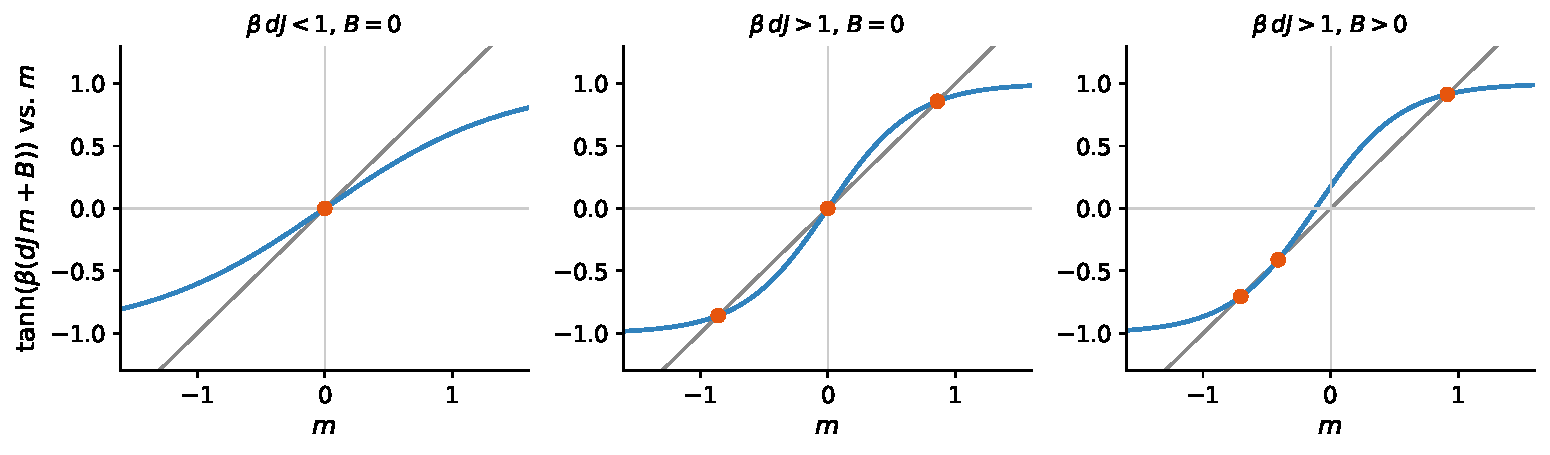
\includegraphics[width=\linewidth]{fig/slides-tanh.pdf}
  \end{center}
  %One symmetric solution; three solutions (two degenerate minima);
  %asymmetric minima.
\end{frame}

%=====================================================================
\begin{frame}{Self-consistency (an aside)}

There's another path to the saddle-point equation. Look at the effective field/force felt by a single $\theta_i$:
%
\[  B^{\rm eff} = - \partial_{\theta_i} E(\theta) = J \sum_{j\sim i} \theta_j + B \approx  dJ m+B\,. \]
\vspace{-.3cm}

The partition function for a single $\theta_i$ in this effective field becomes
%
\[ Z_i = \sum_{\theta_i=\pm 1} e^{\beta B^{\rm eff} \theta_i} = 2\cosh\beta B^{\rm eff} = 2\cosh \beta(dJm+B)\,. \]
%
If the mean-field approx. is consistent, we'd better find
%
\[   m \overset{!}= \mathbb E(\theta_i) = \tfrac{1}{\beta} \partial_B \log Z_i = \tanh \beta(dJ m+B) \]
\emph{I.e.} the average that comes \emph{out} to equal the average we
  put in!
\end{frame}

%=====================================================================
\begin{frame}{Phases \& phase transitions}
  Analyze the structure of \hl{minima of $s(m)$} --- they control where
  the probability density accumulates. Rich structure as $\beta, J, B$
  are varied! Taylor-expanding $h(m) \approx \log 2 - \frac{m^2}{2}
  - \frac{m^4}{12}$:
  \[
    s(m) \;\approx\; \mathrm{const} - B\,m
    + \tfrac12\big(\beta^{-1} - Jd\big)\, m^2
    + \tfrac{\beta^{-1}}{12}\, m^4 + \cdots
  \]
  Take $Jd > \beta^{-1}$ (coupling beats temperature: the system tries to
  be \emph{ordered}, neighboring spins align. But which way?)
  \begin{center}
    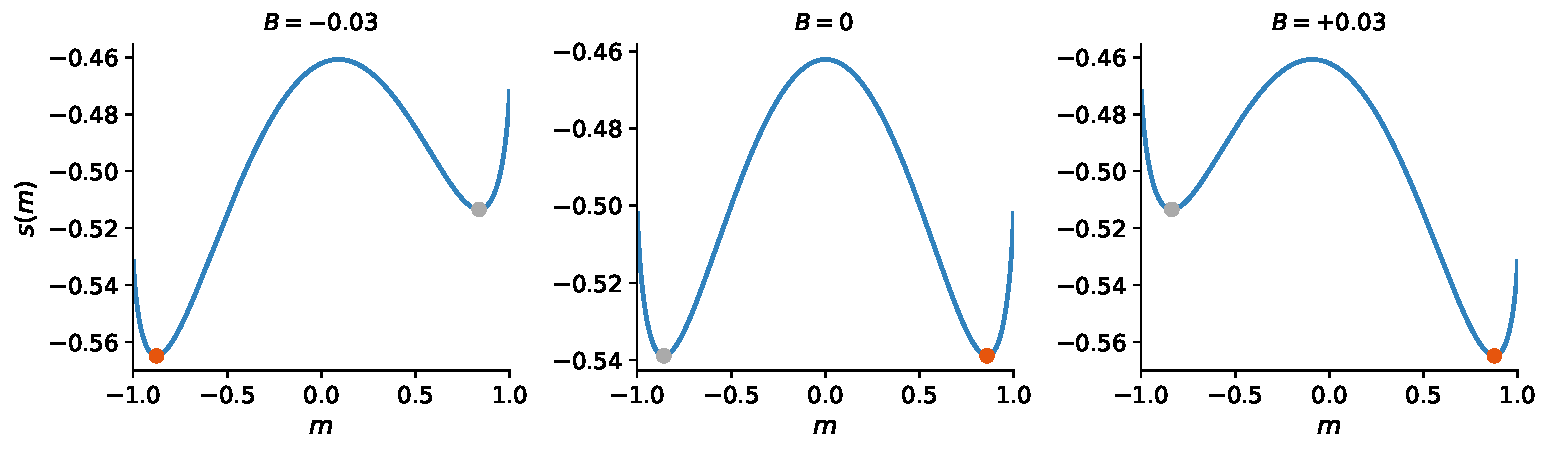
\includegraphics[width=0.95\linewidth]{fig/slides-wells.pdf}
  \end{center}
  They align \hl{with the magnetic field $B$}: \ $\bar m \approx -1$ for
  $B<0$, \ $\bar m \approx +1$ for $B>0$.
  This is a \hl{first-order phase transition} as $B$ crosses $B_c = 0$.
\end{frame}

%=====================================================================
\begin{frame}{Features of a first-order transition}
  The structure of this transition, as two isolated minima cross, is universal (independent of the model). Look at $\E(m) = \frac{1}{N\beta}\frac{\pd F}{\pd B}$:  \begin{center}
    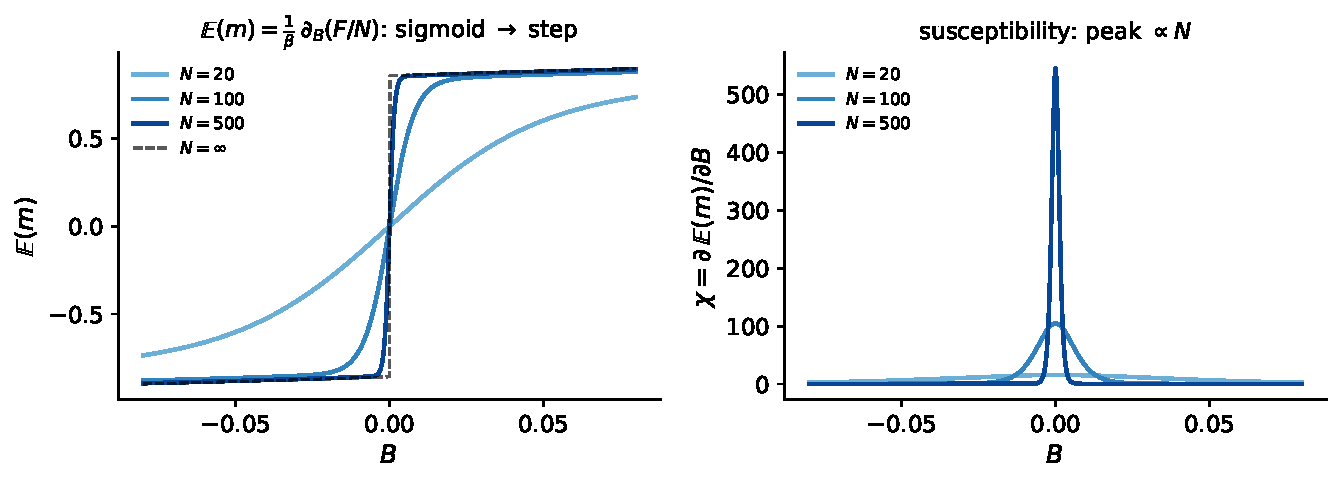
\includegraphics[width=0.9\linewidth]{fig/slides-firstorder.pdf}
  \end{center}
  As $N\to\infty$, the saddle-point approx. strongly prefers $m$ to sit in the lowest minimum, so $\mathbb E(m) =\beta^{-1} \partial_B (F/N)$ develops a discontinuity ---  the
  \emph{definition} of a first-order phase transition.
  The ``susceptibility'' $\chi := \pd_B \E(m) = \beta^{-1} \pd_B^2(F/N)$
  diverges to a $\delta$.
\end{frame}

%=====================================================================
\begin{frame}{A second-order transition, too}
  An \emph{$n$-th order} phase transition $=$ discontinuity in the $n$-th
  derivative of $F/N$, as $N\to\infty$.
  \vspace{1mm}

  In the Ising model this happens at fixed $B = 0$ (symmetric minima), as the temperature $T = \beta^{-1}$ crosses $T_c = Jd$:
  \begin{center}
    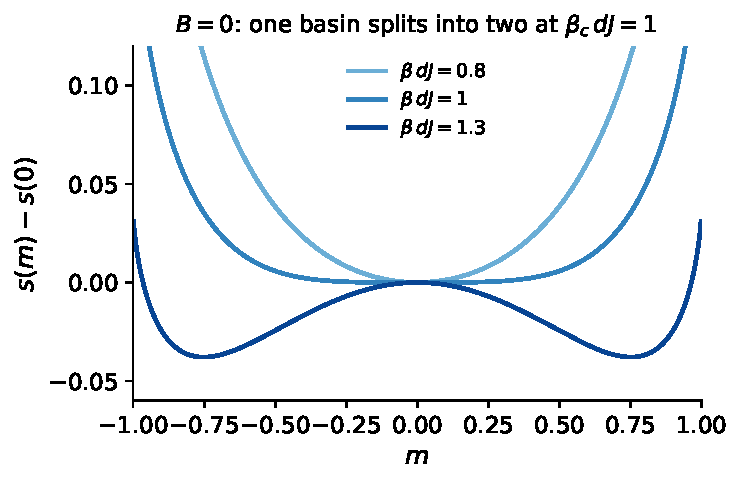
\includegraphics[width=0.62\linewidth]{fig/slides-secondorder.pdf}
  \end{center}
  One basin deforms and splits: the order parameter $\E(m)$ moves
  \emph{continuously} but not smoothly ($\E(m) \propto (\beta-\beta_c)^{1/2}$).
\end{frame}

%=====================================================================
\begin{frame}{Back to learning: Bayes vs.\ gradient descent}
  We don't train networks with Bayesian learning; we train them with
  \hl{gradient descent}. Recall the expected analogy:
  \[
    (*)\qquad
    \underbrace{n \to \infty}_{\text{samples / learning time}}
    \;\;\rightsquigarrow\;\;
    \beta \to \infty \quad (T \to 0)\,.
  \]
  \begin{itemize}
    \item In Ising, this sweep would see the \emph{second}-order transition.
    \item For \emph{first}-order transitions, when we \emph{dynamically}
      vary a parameter there is \hl{hysteresis}: transitions are
      delayed. (One dynamical analogue in neural networks: the
      MSRJD formalism $+$ DMFT --- not in these lectures!)
  \end{itemize}
\end{frame}

%=====================================================================
\begin{frame}{The Langevin equation (an aside)}
  Another connection to gradient descent, worth knowing: the
  \hl{Langevin equation}
  \[
    \dot\theta = -\nabla_\theta L(\theta) + T^{1/2}\, d\xi
    \qquad (\text{Gaussian noise, variance $T$})\,.
  \]
  \begin{itemize}
    \item Starting from any sufficiently generic prior, at late training time ($t\to \infty$) this
      converges to $p(\theta) \propto e^{-\frac1T L(\theta)}$: one can
      ``Bayesian train'' a network in practice.
      
      (More on this in Tong's \emph{Kinetic Theory} lectures.)
    \item Alternatively, $T\to0$ at finite time $t$ produces gradient flow $\dot\theta = -\nabla_\theta L$.
    
    \medskip
    $\leadsto$ a \emph{different} Bayesian $\leftrightarrow$ gradient connection.
  \end{itemize}
\end{frame}

%=====================================================================
\begin{frame}{Exercises (Part I)}
  See the handout. Do \emph{one} of these.
  
  Alternatively, go through formulas from the lecture and verify them.
  
  \vspace{3mm}
  \begin{enumerate}
    \item[0.] Expectations and cumulants from the free energy.
    \item[1.] \textbf{Anatomy of a first-order transition.} Work out the
      curves $\dfrac{\pd f}{\pd\beta}$ and $-\dfrac{\pd^2 f}{\pd\beta^2}$
      \ ($f = F/N$) for a generic first-order phase transition ---
      and interpret them as the mean energy and the variance of the
      energy (heat capacity).
      \vspace{2mm}
    \item[2.] \textbf{The Ising perceptron.} Your turn! Analyze a simple learning problem and discover a first-order phase transition to perfect generalization.
  \end{enumerate}
  \vspace{4mm}
  \begin{center}
%    \footnotesize Full lecture notes: \emph{Physics of Deep Learning}
%   (Sections 2.3--2.4 expand on today's Part I).
  \end{center}
\end{frame}

%=====================================================================
\begin{frame}{References \& further reading (Part I)}
  \small
  \begin{itemize}
    \item D.~Tong, \emph{Statistical Field Theory} lecture notes ---
      the physics behind this part (and \emph{Kinetic Theory}, for the
      Langevin equation).
    \item A.~Engel and C.~Van den Broeck, \emph{Statistical Mechanics of
      Learning} --- the perceptron tradition; the Ising perceptron
      transition goes back to G.~Gy\"orgyi (1990).
    \item The long lecture notes, \emph{Physics of Deep Learning},
      expand on everything today, with worked solutions.
  \end{itemize}
\end{frame}

%=====================================================================
% PART II
%=====================================================================
\title{Physics of Deep Learning\\[2pt]
\large Part II: Scaling neural networks and feature learning}
\begin{frame}
  \titlepage
  \vspace{-2mm}
  \begin{block}{Main question}
    Given a neural network, analyzed either dynamically (SGD) or via
    equilibrium Bayesian methods: \emph{what scaling limits simplify the
    analysis?} (And are these limits realistic?)
  \end{block}
  \begin{center}\small
  \begin{tabular}{ll}
    1. & Lazy scaling at initialization \\
    2. & Detour/reminder: the NTK \& features \\
    3. & Lazy scaling during training \\
    4. & Mean-field scaling (and $\mu$P)
  \end{tabular}
  \end{center}
\end{frame}

%=====================================================================
\begin{frame}{Setup: the MLP}
  A network with parameters $\theta\in\R^P$. Keep it simple: an
  \hl{MLP} (fully-connected network), input $x \in \R^d$, $L$ hidden
  layers each of width $N$, one output $f(x)$.
  \vspace{2mm}

  Pre-activations in layer $\ell$:
  \[
    z^{(\ell)}_i = \sum_{j=1}^{N} w^{(\ell)}_{ij}\, \phi\big(z^{(\ell-1)}_j\big)\,,
    \quad\text{except}\quad
    z^{(1)}_i = \sum_{j=1}^{d} w^{(1)}_{ij}\, x_j \ \ (\text{no } \phi)\,,
  \]
  \[
    f = z^{(L+1)} \qquad\text{so}\qquad
    \theta = \{w^{(1)}, \dots, w^{(L+1)}\}\,.
  \]
  \vspace{1mm}

  (No biases --- they don't add anything conceptual.)
\end{frame}

%=====================================================================
\begin{frame}{Randomness at initialization}
  There is already randomness here, from random initialization:
  $\theta \sim \pi(\theta)$ (some \emph{prior}).
  \vspace{2mm}

  \hl{Question:} how does the randomness propagate to the values
  $f_\theta(x)$? Specifically: given the distribution $\pi$ on
  $\theta$'s and fixed inputs $x^1, \dots, x^k \in \R^d$, what is the
  \hl{push-forward distribution} on
  \[
    \big(f(x^1),\, \dots,\, f(x^k)\big)\ ?
  \]
  \vspace{1mm}

  This simplifies greatly as $N\to \infty$.
  \vspace{1mm}

  But exactly \emph{how} it simplifies depends strongly on $\pi$ (as well as how learning rate, $L$, etc. scale with $N$).
\end{frame}

%=====================================================================
\begin{frame}{Lazy initialization (``fan-in norm'')}
  \hl{Lazy init:} try to keep all pre-activations $z^{(\ell)} = O(1)$.
  \[
    z^{(\ell)}_i = \sum_{j=1}^{N} \underbrace{w^{(\ell)}_{ij}}_{N\ \text{random coeffts}}
    \underbrace{\phi\big(z^{(\ell-1)}_j\big)}_{O(1)}
  \]
  \[
    \Longrightarrow\quad
    \text{take}\ \ w^{(\ell)}_{ij} \sim \frac{1}{\sqrt N}\,,\qquad
    w^{(1)}_{ij} \sim \frac{1}{\sqrt d}\,.
  \]
  Let's implement this explicitly: for $\ell>1$ set
  \[
    z^{(\ell)}_i = \frac{1}{\sqrt N}\sum_{j=1}^N w^{(\ell)}_{ij}\,
    \phi\big(z^{(\ell-1)}_j\big)\,,
    \qquad w^{(\ell)}_{ij} \sim \mathcal N(0,1)\,,
  \]
  so all the weights are now of order one.
\end{frame}

%=====================================================================
\begin{frame}{Gaussian processes}
  \textbf{Definition.} Given $\mu: \R^d \to \R$ and
  $K: \R^d\times\R^d \to \R$ (the \hl{kernel}), a \hl{Gaussian process}
  is a random function $f: \R^d \to \R$ such that for any
  $(x^1, \dots, x^k)$, the joint distribution of
  $\big(f(x^1), \dots, f(x^k)\big)$ is Gaussian with mean
  $\big(\mu(x^1), \dots, \mu(x^k)\big)$ and covariance matrix
  \[
    \begin{pmatrix}
      K(x^1,x^1) & \cdots & K(x^1,x^k) \\
      \vdots & & \vdots \\
      K(x^k,x^1) & \cdots & K(x^k,x^k)
    \end{pmatrix}.
  \]
  \vspace{1mm}

  Equivalently: mean and covariance exist, but \emph{all higher
  cumulants vanish} (recall the cumulants of Part I --- here the
  observables are the $f(x^i)$ themselves).
\end{frame}

%=====================================================================
\begin{frame}{Theorem: lazy init $\Rightarrow$ Gaussian process}
  \textbf{Theorem} (Neal; Lee et al.; Yang; Hanin\dots).
  Fix $L$ and $x$'s. With lazy init, as $N \to \infty$, $f$ converges to
  a Gaussian process, with recursively defined kernel:
  \[
    K^{(\ell+1)}(x,x') =  \E_{z\,\sim\, K^{(\ell)}}
    \Big[\phi\big(z(x)\big)\,\phi\big(z(x')\big)\Big]\,,
  \]
  with base case $K^{(1)}(x,x') =  \frac{1}{d}x\cdot x'$.
  \emph{Sketch:} the first layer is a sum of Gaussians --- exactly
  Gaussian, with kernel $K^{(1)}$. Induct on layers:
  \emph{conditioned} on layer $\ell$, the $z^{(\ell+1)}_i$ are i.i.d.\
  Gaussian with the \emph{random} kernel
  $\widehat K^{(\ell)} = \frac{1}{N}\sum_j
  \phi(z_j^{(\ell)}(x))\,\phi(z_j^{(\ell)}(x'))$.
  Key: as $N\to\infty$ its variance $\to 0$, so it becomes
  \emph{deterministic} --- and Gaussianity propagates.
  \vspace{2mm}

  The recursion has an analytic form for $\phi = \mathrm{ReLU}$ and
  $\mathrm{erf}$.
  \vspace{1mm}

  {\footnotesize (There is also a slick physics derivation by path
  integrals --- left as an exercise for those who like them; see the
  long notes, \S3.)}
\end{frame}

%=====================================================================
\begin{frame}{Proof sketch, I: the first layer is exactly Gaussian}
  Fix the inputs $x^1, \dots, x^k$. The first layer, with the
  $1/\sqrt d$ explicit, is
  \[
    z^{(1)}_i(x) = \frac{1}{\sqrt d}\sum_{j=1}^{d} w^{(1)}_{ij}\, x_j\,,
    \qquad w^{(1)}_{ij} \sim \mathcal N(0,1)\ \ \text{i.i.d.}
  \]
  For fixed $i$, this is a linear combination of independent Gaussians
  with \emph{fixed} coefficients $x_j/\sqrt d$ --- so
  $\big(z^{(1)}_i(x^1), \dots, z^{(1)}_i(x^k)\big)$ is \hl{exactly
  jointly Gaussian} (no large-$N$ limit needed), with mean zero and
  kernel
  {\small
  \[
    K^{(1)}(x,x') = \E\big[z^{(1)}_i(x)\, z^{(1)}_i(x')\big]
    = \frac1d \sum_{j,j'=1}^{d} x_j\, x'_{j'}\,
    \underbrace{\E\big[w^{(1)}_{ij} w^{(1)}_{ij'}\big]}_{
    \delta_{jj'}}
    =  \frac{x\cdot x'}{d}\,.
  \]}
  Moreover, distinct neurons $i \neq i'$ use \emph{disjoint} sets of
  weights, so the $z^{(1)}_i$ are i.i.d.\ across $i$: layer 1 is $N$
  independent copies of one Gaussian process.
\end{frame}

%=====================================================================
\begin{frame}{Proof sketch, II: induction on layers}
  \emph{Inductive hypothesis:} as $N\to\infty$, the $z^{(\ell-1)}_j$
  become i.i.d.\ GPs with deterministic kernel $K^{(\ell-1)}$.

  \hl{Conditioned} on layer $\ell-1$, the coefficients
  $\phi\big(z^{(\ell-1)}_j\big)$ are frozen, so
  $z^{(\ell)}_i = \frac{1}{\sqrt N}\sum_j w^{(\ell)}_{ij}\,
  \phi\big(z^{(\ell-1)}_j\big)$ is \emph{again} linear in Gaussian
  weights: exactly Gaussian, i.i.d.\ across $i$, with kernel
  {\small
  \[
    \widehat K^{(\ell)}(x,x') = \frac{1}{N}\sum_{j=1}^{N}
    \phi\big(z^{(\ell-1)}_j(x)\big)\,\phi\big(z^{(\ell-1)}_j(x')\big)\,.
  \]}
  \emph{Un}-conditionally, $\widehat K^{(\ell)}$ is a \hl{random
  variable} --- but an average of $N$ i.i.d.\ $O(1)$ terms (by the
  inductive hypothesis), so
  $\mathrm{Var}\big[\widehat K^{(\ell)}\big] = O\big(\tfrac1N\big)$,
  with mean
  {\small
  \[
    \E\big[\widehat K^{(\ell)}\big]
    =  \E_{z \sim K^{(\ell-1)}}
    \big[\phi\big(z(x)\big)\,\phi\big(z(x')\big)\big]
    = K^{(\ell)}(x,x')\,.
  \]}
  \hl{Key:} as $N\to\infty$ the variance $\to 0$: the kernel becomes
  \emph{deterministic}. A Gaussian mixture with deterministic kernel is
  Gaussian --- and the neurons, coupled only through
  $\widehat K^{(\ell)}$, stay independent: Gaussianity propagates.
\end{frame}

%=====================================================================
\begin{frame}{Lesson --- and the $L/N$ expansion}
  \hl{Lesson:} the $N\to\infty$ limit with lazy init is \emph{boring} (but tractable!) at
  init. It also turns out boring(ish) in training.
  \vspace{1mm}

  \hl{But:} the $N\to\infty$ limit does \emph{not} commute with
  $L\to\infty$. If $L$ is large, each successive layer gets larger
  fluctuations in its kernel, and they don't die off.
  \vspace{1mm}

  Hanin, Roberts--Yaida: for $N, L \to\infty$ networks the relevant
  expansion parameter is $\boxed{L/N}$. We've just analyzed $L/N = 0$.
  \begin{itemize}
    \item \emph{Small} (but nonzero) $L/N$: no longer Gaussian ---
      cumulants $K^{(4)}(f(x^1), \dots, f(x^4))$ nonzero, but
      \emph{controllable}.
    \item \emph{Large} $L/N$: each successive cumulant is even larger;
      uncontrollable outputs.
  \end{itemize}
  \vspace{1mm}

  This translates to \hl{training} (SGD, GD, grad flow, even Bayesian):
  \begin{center}
  \begin{tabular}{ll}
    $\tfrac LN = 0$: & network is linear (features fixed); \\
    $\tfrac LN$ small: & features can be learned; \\
    $\tfrac LN$ large: & chaotic, divergent flows $\to$ untrainable network.
  \end{tabular}
  \end{center}
%  (Where do real models sit? Exercise 0.)
\end{frame}

%=====================================================================
\begin{frame}{Detour: gradient flow and the NTK}
  To analyze training and quantify ``features'', we'll introduce a geometric object known as the Neural Tangent Kernel (NTK).
  
  (Jacot, Gabriel, Hongler 2018)

\bigskip

  \emph{Recall:} on a manifold $X$ with smooth $h: X\to\R$ and a
  non-degenerate metric $g = g_{ab}(x)\,dx^a dx^b$, \hl{gradient flow}
  is
  \[
    \frac{dx^a}{dt} = -\,g^{ab}(x)\,\frac{\pd h}{\pd x^b}
    \qquad\text{(the flow of the vector field } -g^{-1}(dh)\text{)}\,.
  \]
  You \emph{need} a metric to define gradient flow, descent, etc.
  \vspace{2mm}

  In the parameter space of neural networks, the metric is assumed to be
  \hl{Euclidean}: $g_\theta = \delta_{ij}\, d\theta^i d\theta^j$.
  \ (First source of inductive bias!)
  \vspace{1mm}

  Training (as gradient flow) is $\ \dot\theta^i = -\,\delta^{ij}\pd_j L(\theta)$.
\end{frame}

%=====================================================================
\begin{frame}{Push the flow to function space: the NTK}
  Suppose $\{x^\mu\}_{\mu=1}^n$ are fixed inputs, with network outputs
  $f^\mu = f_\theta(x^\mu)$ and ``truth'' values $y^\mu$. Push forward
  the flow from $\theta\in\R^P$ to $\{f^\mu\}\in\R^n$: the standard
  coordinate transformation of the \emph{inverse metric} gives
  \[
    \delta^{ij}\ \text{on}\ \R^P
    \quad\rightsquigarrow\quad
    \Theta^{\mu\nu} = \frac{\pd f^\mu}{\pd\theta^i}\,\delta^{ij}\,
    \frac{\pd f^\nu}{\pd\theta^j}
    = \nabla_\theta f^\mu \cdot \nabla_\theta f^\nu\ \text{on}\ \R^n\,,
  \]
  \[
    \dot\theta = -\nabla_\theta L
    \quad\rightsquigarrow\quad
    \dot f^\mu = - \,\underbrace{\Theta^{\mu\nu}}_{\text{\hl{NTK}}}\ \underbrace{\pd_{f^\nu} L}_{\text{residual}}\,.
  \]
  Compactly, $\Theta = J J^{\!\top}$ with $J = \nabla_\theta f$ the
  Jacobian.
  
   For MSE loss
   \[ L = \frac12\sum_\mu |f^\mu - y^\mu|^2\quad\Rightarrow\quad
  \pd_{f^\mu}L = f^\mu - y^\mu =: \Delta^\mu \,. \] 

  \emph{``The NTK controls the geometry of optimization.''}
\end{frame}

%=====================================================================
\begin{frame}{Features, via the SVD}
  At a given $\theta$, the Jacobian $J$ says how the network values (on
  training data) respond to a shift in parameters. Take its SVD:
  \[
    J = U\,\Lambda\, V^{\!\top}\,,\qquad
    \Lambda = \big(\,\mathrm{diag}(\sqrt{\lambda_1}, \sqrt{\lambda_2},
    \dots)\ \big|\ 0\,\big)\,.
  \]
  \begin{itemize}
    \item columns of $V$: modes in \emph{parameter} space;
    \item columns of $U$: modes in \emph{function values} $\to$
      \hl{``features''};
    \item $\Theta = JJ^{\!\top} = U\,\Lambda\Lambda^{\!\top} U^{\!\top}$:
      the features are the \hl{eigenvectors of the NTK}, with
      eigenvalues $\lambda_k$.
  \end{itemize}
  \vspace{2mm}

  This is a commonly used theoretical notion of \emph{feature}.
  
  \medskip
  \emph{Cf.} Activation-space or SAE features, grokked capabilities...
  \vspace{2mm}

  {\footnotesize \hl{An empirical comparison:} see J.~Lin,
  \emph{Feature Identification via the Empirical NTK},
  arXiv:2510.00468: NTK eigenvectors matching features actually learned in modular arithmetic and a small language model.}
\end{frame}

%=====================================================================
\begin{frame}{How big is the NTK, in lazy scaling?}

Back to training at large $N$! What does the NTK look like?

\medskip

  Try $L = 1$:\quad
  $\displaystyle f(x) = \frac{1}{\sqrt N}\sum_{i=1}^N c_i\,\phi(a_i\cdot x)$,
  \quad $a, c \sim \mathcal N(0,1)$.
  \[
    \nabla f = \frac{1}{\sqrt N}\bigoplus_i \Big(\phi(a_i\cdot x)\,,\
    c_i\,\phi'(a_i\cdot x)\, x\Big)
  \]
  \vspace{-.3cm}
  {\small
  \[
    \Theta^{\mu\nu} = \frac1N \sum_{i=1}^N
    \Big[\phi(a_i\cdot x^\mu)\,\phi(a_i\cdot x^\nu)
    + c_i^2\,\phi'(a_i\cdot x^\mu)\,\phi'(a_i\cdot x^\nu)\;
    x^\mu\!\cdot x^\nu\Big] = O(1)\,.
  \]}
  Similarly, at finite depth $L$ and large $N$ (with the $1/\sqrt N$'s
  explicit): $\Theta = $ sum of $L$ terms, each $O(1)$ --- so
  $\Theta = O(1)$, positive-definite.
  \vspace{2mm}

  {\footnotesize \hl{Warning:} in the $w \sim \mathcal N(0, \frac1N)$ parametrization one
  finds $\Theta = O(N)$; the order-one flow there is
  $\dot\theta = -\frac{\eta}{N}\nabla L$. Rescaling parameters rescales
  the metric on parameter space --- think of it as rescaling the
  \emph{learning rate}. What matters: $O(1)$ changes in $f^\mu$; figure
  out the size of $\Theta$ and scale $\eta$ accordingly.}
\end{frame}

%=====================================================================
\begin{frame}{Theorem: lazy training is lazy}
  \textbf{Theorem} (Du et al., Jacot et al., \dots). Fix depth, data,
  and a sufficiently overparametrized lazy network, trained by gradient
  flow with the scalings above. Despite the fact that $f^\mu = O(1)$
  moves and fits the data:
  \begin{itemize}
    \item The network \hl{linearizes} around initialization:
      \[
        f_\theta(x) = f_{\theta_0}(x)
        + (\theta - \theta_0)\cdot \nabla_\theta f(x)\big|_{\theta_0}
        + O\Big(\tfrac{1}{\sqrt N}\Big)\,;
      \]
    \item the NTK \hl{freezes}:
      $\displaystyle \frac{\|\dot\Theta\|}{\|\Theta\|} =
      O\Big(\frac{1}{\sqrt N}\Big)\,;$
    \medskip
    \item $f(x^\mu) \to y^\mu$ \emph{exponentially fast} in training
      time, with rates determined by the spectrum of $\Theta$.
  \end{itemize}
\end{frame}

%=====================================================================
\begin{frame}{Why? (sketch)}
  \begin{enumerate}
    \item $\|\nabla^2 f\|_{\rm op} = O\big(\tfrac{1}{\sqrt N}\big)$: a
      big matrix, but \emph{sparse} --- block-diagonal per neuron, each
      block carrying the explicit $\tfrac{1}{\sqrt N}$. (In fact
      $O(\tfrac1N)$ after cancelling fluctuations, but $\tfrac{1}{\sqrt
      N}$ is enough.)
    \item Taylor-expand: the quadratic term is
      $\|\Delta\theta\|^2\,\|\nabla^2 f\|_{\rm op} \approx O(1)\times
      O\big(\tfrac{1}{\sqrt N}\big)$, using $\|\Delta\theta\| =
      O(1)$ from $\|\dot\theta\| = \|\sum_\mu \Delta^\mu \nabla f^\mu\|
      \sim \sqrt{\Theta} = O(1)$.
    \item $\|\dot\Theta\| \leq 2\,\|\nabla^2 f\|_{\rm op}\,
      \|\dot\theta\|\,\|\nabla f\| \to 0$: the kernel freezes.
    \item With $\Theta$ constant, the flow solves itself:
      $\dot\Delta^\mu = -\Theta^{\mu\nu}\Delta_\nu$, so in the
      NTK eigenbasis ($\Theta = U\Lambda\Lambda^\top U^\top$)
      \[
        (U^{\!\top}\Delta)_k(t) = e^{-\lambda_k t}\,
        (U^{\!\top}\Delta)_k(0)\,:
      \]
      the $k$-th mode/feature is learned in  time
      $\boxed{t_k \approx 1/\lambda_k}$.
  \end{enumerate}
\end{frame}

%=====================================================================
\begin{frame}{Lazy learning $=$ kernel regression}
  This is called \hl{lazy learning}: it uses the (\emph{random}!)
  features from initialization to approximate the actual features in the
  data. Overparametrized system, so that's fine --- but it only
  \emph{memorizes}.
  \vspace{1mm}

  {\footnotesize [The learning algorithm here is simple and well known:
  \emph{kernel regression}.]}
  \vspace{4mm}

  This is \hl{not} a good model for actual neural networks, which
  \emph{change} their NTK (phase transitions!) to adapt to the training
  data and generalize intelligently.
  
  Remarkably, it's enough to predict some basic behavior (Part III).
  
  \vspace{3mm}

  Theoretical setups that do better? Yes! Simplest options:
  \begin{itemize}
    \item small $L/N > 0$ \ [see e.g.\ Roberts--Yaida--Hanin];
    \item a \emph{different init}: we'll look at \hl{mean-field
      scaling}
      
      \smallskip
      {\footnotesize[Generalized to $\mu$P (maximal-update
      param.), Yang \& Hu 2019]}
  \end{itemize}
\end{frame}

%=====================================================================
\begin{frame}{Mean-field scaling}
  For an $L=1$ network, change $\dfrac{1}{\sqrt N} \to \dfrac1N$:
  \[
    f(x) = \frac1N \sum_{i=1}^N c_i\,\phi(a_i\cdot x)\,,\qquad
    c_i,\, a_{ij} \sim \mathcal N(0,1)\,,
  \]
  and send $N\to\infty$. Main differences from the lazy regime:
  \begin{itemize}
    \item At init, $f(x) \to 0$: the Gaussian process \emph{collapses}.
    \item In training, $\Theta^{\mu\nu} = O\big(\tfrac1N\big)$ ---
      which \emph{forces} the learning rate to scale as $N$ for anything to happen:
      \[
        \dot\theta = -N\,\nabla_\theta L\,,\qquad
        \dot f^\mu = -N\,\Theta^{\mu\nu}\Delta^\nu\,.
      \]
  \end{itemize}
  $\rightsquigarrow$ a nonlinear (in parameters) network, with an
  \hl{adaptive NTK}. Why does the NTK move now?
  \[
    \frac{|\dot\Theta|}{|\Theta|} \;\lesssim\;
    \underbrace{N}_{\text{l.r.}}\cdot\,
    \|\nabla^2 f\|_{\rm op}
    = N\cdot O\Big(\tfrac{1}{\sqrt N}\!\cdot\!\tfrac{1}{\sqrt N}\Big) = O(1)\,,
  \]
  so it \emph{can} move; a closer analysis of $\dot a_i, \dot c_i$ shows that it \emph{does}.
\end{frame}

%=====================================================================
\begin{frame}{Why the name ``mean field''?}
  Think of $(a_i, c_i)_{i=1}^N$ as parameters for \hl{$N$ particles},
  each contributing $g^\mu_i := c_i\,\phi(a_i\cdot x^\mu)$ to
  $f(x^\mu)$. The loss/energy is
  \[
    L = \frac12\sum_{\mu=1}^n \big(f(x^\mu) - y^\mu\big)^2
    = \frac1N \sum_{\mu=1}^n \Big[\frac{1}{2N}\sum_{i,j=1}^N
    g^\mu_i\, g^\mu_j
    - y^\mu \sum_{i=1}^N g^\mu_i\Big] + \text{const}
  \]
  \emph{Same form as the mean-field approximation of Ising!} Weak
  all-to-all couplings, depending only on the \hl{averages}
  \[
    G^\mu = \frac1N\sum_i g^\mu_i\,:\qquad
    L = \cancel{\frac1N} \cdot N \sum_\mu \Big[\tfrac12 (G^\mu)^2 - y^\mu
    G^\mu\Big]\,.
  \]
  \textbf{Theorem.} As $N\to\infty$, at all training times $t$, the
  distribution of particles converges,
  \[
    {\frac1N}\sum_i \delta(a - a_i)\,\delta(c - c_i)
    \;\longrightarrow\; \mu_t(a,c)\,:
  \]
  a \emph{smooth, deterministic} measure obeying a deterministic PDE.
  {\footnotesize (Details, and a Bayesian attack on the same system:
  long notes, \S5.)}
\end{frame}

%=====================================================================
\begin{frame}{Feature learning, watched directly}
  \begin{center}
    \includegraphics[width=0.98\linewidth]{fig/mf-transport.pdf}
  \end{center}
  Training in mean-field scaling transports the \emph{cloud of neurons}
  $(a_i, c_i)$ (left: dots colored by time, over the large-$N$ density),
  which condenses onto the low-dimensional structures realizing the
  target --- learning its features --- while the network function
  converges (right). This is the model of Exercise 2.
\end{frame}

%=====================================================================
\begin{frame}{Exercises (Part II)}
  See the handout:
  \vspace{2mm}
  \begin{enumerate}
    \setcounter{enumi}{-1}
    \item \textbf{Depth-to-width ratios in the wild.} Look up $L/N$ for
      open-weight LLM families: is everyone training in the
      ``controlled correlations'' window?
      \vspace{1mm}
    \item \textbf{Bayesian lazy learning.} The Bayesian-learning version
      of the lazy story: eigenmodes of the GP kernel at init are learned
      with characteristic ``time'' $\beta_k = 1/\lambda_k$ --- the
      equilibrium twin of $t_k = 1/(\eta\lambda_k)$.
      \vspace{1mm}
    \item \textbf{Numerics: lazy vs.\ mean-field.} Train one small
      network in both scalings. Watch the NTK freeze in one and move in
      the other, and watch the particle cloud $(a_i, c_i)$ condense onto
      features.
  \end{enumerate}
\end{frame}

%=====================================================================
\begin{frame}{References \& further reading (Part II)}
  \small
  \begin{itemize}
    \item B.~Hanin, \emph{Mathematics of Deep Learning} lectures --- large $N$\\
      {\footnotesize \url{https://www.youtube.com/watch?v=4SVWo5kspR8}}
    \item D.~Roberts, S.~Yaida, and B.~Hanin, \emph{The Principles of
      Deep Learning Theory} --- the $L/N$ expansion.
    \item Z.~Ringel, N.~Rubin, E.~Mor, M.~Helias, and I.~Seroussi,
      \emph{Applications of Statistical Field Theory in Deep Learning}.
    \item K.~Spiliopoulos, R.~Sowers, and J.~Sirignano,
      \emph{Mathematical Foundations of Deep Learning Models and
      Algorithms} --- mean-field limits.
    \item The long lecture notes, \emph{Physics of Deep Learning},
      \S3--\S5, with worked solutions.
  \end{itemize}
\end{frame}

%=====================================================================
% PART III
%=====================================================================
\title{Physics of Deep Learning\\[2pt]
\large Part III: Neural scaling laws}
\begin{frame}
  \titlepage
  \vspace{-2mm}
  \begin{block}{Organizing question}
    The test loss of large models falls as a clean power law in every
    resource spent on it. \ \emph{Where do the exponents come
    from?}
  \end{block}
\end{frame}

%=====================================================================
\begin{frame}{The empirical laws (Kaplan et al.\ 2020)}
  For autoregressive language models, when not bottlenecked by the other
  resources, test loss obeys
  \[
    L(N) \propto N^{-\alpha_N}\,,\qquad
    L(D) \propto D^{-\alpha_D}\,,\qquad
    L(C) \propto C^{-\alpha_C}\,,
  \]
  with
  \begin{itemize}
  \item \hl{$N$} $=$ parameters (non-embedding)
  \item \hl{$D$} $=$ dataset size (in tokens)
  \item $C$ $=$ training compute (in FLOPs).
  \end{itemize}
  (Note: for single-epoch training, $C\approx 6ND$, with $N$ \& $D$ optimally allocated.)
   %
 % \footnote{\emph{Why $6ND$:} forward $\approx 2N$ FLOPs/token (one
  %multiply--add per parameter); backward $\approx 2\times$ forward
  %(gradients w.r.t.\ activations \emph{and} weights): $6N$ per token,
  %$\times D$ tokens. \emph{Why FLOPs, not steps/time:} FLOPs are
  %batch-size-, hardware-, and parallelism-independent. (The long notes
  %write $P, n$ for $N, D$.)}
  
  \medskip
  Measured exponents, holding over many orders of magnitude:
  \begin{center}
    $\alpha_N \approx 0.076\,,\qquad
    \alpha_D \approx 0.095\,,\qquad
    \alpha_C \approx 0.050\,.$
  \end{center}
 % \begin{center}
 %   \includegraphics[width=0.8\linewidth]{fig/slides-kaplan.pdf}
 % \end{center}
\end{frame}

%=====================================================================
\begin{frame}{Universal form; data-dependent exponents}
  The same power-law \emph{form} holds across modalities (Henighan et
  al.\ 2020) --- but the \emph{exponents} follow the data:
  \begin{center}\small
  \begin{tabular}{l|cc}
    modality & $\alpha_N$ & $\alpha_C$ \\\hline
    language & $0.070$ & $0.048$ \\
    images $32{\times}32$ & $0.13$ & $0.10$ \\
    images $8{\times}8$ & $0.24$ & $0.19$ \\
    video & $0.24$ & $0.14$ \\
    math (procedural) & $0.16$ & $0.17$
  \end{tabular}
  \end{center}
  \vspace{1mm}
  \begin{itemize}
    \item \hl{Data matters}: exponents vary by a factor of
      $\sim\!3$--$5$ across modalities. 
      %(Preview: Sharma--Kaplan explain
      %this as $\alpha_N \approx 4/d$, $d =$ \emph{intrinsic dimension}
      %of the data manifold --- language is high-$d$, hence slow.)
    \item \hl{Architecture barely matters}: within reasonable
      architectures, changing shape (depth vs.\ width) or family moves
      constants and plateaus, not exponents. Whatever sets the exponent
      lives in the \emph{data}.
  \end{itemize}
\end{frame}

%=====================================================================
\begin{frame}{Joint laws and bottlenecks}
  Single-resource laws assume the \emph{other} resources are unlimited.
  Joint fits describe the crossover to being \hl{bottlenecked}: loss is
  governed by whichever resource is scarcest. Two proposals:
  \vspace{1mm}

  \hl{Kaplan et al.:}\quad
  $\displaystyle
    L(N, D) = \Big[\Big(\tfrac{N_c}{N}\Big)^{\alpha_N/\alpha_D}
    + \tfrac{D_c}{D}\Big]^{\alpha_D}
  $
  \vspace{1mm}

  \hl{Chinchilla} (Hoffmann et al.\ 2022):\quad
  $\displaystyle
    L(N, D) = E + \frac{N_c}{N^{\alpha_N}} + \frac{D_c}{D^{\alpha_D}}
    %L(N, D) = E + \frac{A}{N^{0.34}} + \frac{B}{D^{0.28}}
  $
  \vspace{1mm}

  \begin{itemize}
    \item $E$: data's intrinsic noise floor, irreducible entropy \\ ($\approx 1.69$ for text)
    \item Both forms reduce to single-resource power laws as either $N$ or $D$ $\to\infty$, removing bottleneck.
    \item The difference matters for compute-optimal scaling: at fixed $C\approx 6ND$, how to balance $N$ and $D$?
  \end{itemize}
\end{frame}

%=====================================================================
\begin{frame}{Compute-optimal scaling: Kaplan vs.\ Chinchilla}
  %Minimize $L$ at fixed compute $C \approx 6ND$: how should $N, D$ grow?
  \begin{center}
  \begin{tabular}{l|l}
    Kaplan et al.\ 2020 & $N \propto C^{0.73}$, \ $D \propto C^{0.27}$:
    \emph{grow the model} \\
    Chinchilla 2022 &  $N \propto C^{0.5}$, \ $D \propto C^{0.5}$:
    %$N \propto C^{0.5}$, \ $D \propto C^{0.5}$:
    \emph{grow both equally} \\
    & (rule of thumb: $\sim 20$ tokens per parameter)
  \end{tabular}
  \end{center}
  \vspace{1mm}

  \hl{Which is right?} Chinchilla's is now the accepted baseline.
 The discrepancy was analyzed \& understood by Porian et al.\ 2024.
  
 %: Kaplan's fit
 % was skewed by last-layer/embedding compute accounting, too-long
 % warmup at small scale, and scale-dependent optimizer tuning; corrected,
 % the two agree.

\medskip

  Note: In practice, frontier models now \emph{over}-train relative to
  Chinchilla (more data per parameter), because smaller models are cheaper at
  \emph{inference} time.
\medskip

  {\footnotesize Name: \emph{Chinchilla} was DeepMind's 70B model ---
  trained with $4\times$ the data of its 280B predecessor \emph{Gopher}
  at the same compute, and beating it.}
\end{frame}

%=====================================================================
\begin{frame}{Where do the laws come from?}
  Basic answer: the loss curve is reading off the \hl{coarse
  distribution of structure in the data}: power laws in, power laws out.
  \vspace{2mm}

  \begin{columns}
    \begin{column}{0.52\linewidth}
      Simplest example: \hl{Zipf's law}. Rank the words of a corpus
      by frequency,  $f(\text{rank } k) \propto 1/k$.
      %, over
      %$\sim\!4$ decades --- a power-law tail of ever-rarer structure.
      
       \medskip
      (Similar: fact mentions, $n$-grams, image features \dots\; $\propto k^{-\alpha}$)
    \end{column}
    \begin{column}{0.46\linewidth}
      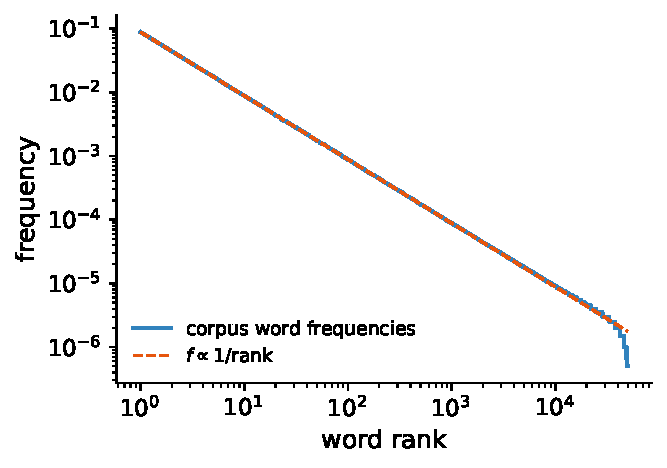
\includegraphics[width=0.88\linewidth]{fig/zipf.pdf}
    \end{column}
  \end{columns}
  \vspace{1mm}

  \hl{Theoretical status:} many models derive the \emph{single-resource} laws from data structure (now fairly clear); a few derive
  \emph{multi-resource} laws. Still missing: the data's exponents from
  first principles; joint laws with full
  feature-learning dynamics; extending to emergent \emph{capabilities}. Also missing theory for empirical RL laws (beyond this lecture).
\end{frame}

%=====================================================================
\begin{frame}{A survey of theoretical proposals}
  \begin{flushleft}
  \tiny
  \renewcommand{\arraystretch}{1.5}
  \setlength{\tabcolsep}{3pt}
  \begin{tabular}{>{\raggedright\arraybackslash}p{1.9cm}|>{\raggedright\arraybackslash}p{2.4cm}|>{\raggedright\arraybackslash}p{2.1cm}|>{\raggedright\arraybackslash}p{1.9cm}|>{\raggedright\arraybackslash}p{1.5cm}}
    \textbf{proposal} & \textbf{data model / ``features''} &
    \textbf{NN framework} & \textbf{exponents?} &
    \textbf{multi-param?} \\\hline
    Sharma--Kaplan 2020 & smooth target on $d$-dim.\ manifold &
    piecewise-linear interpolation & yes: $\alpha_N \approx 4/d$ & no
    ($N$ only) \\
    kernel eigenlearning; Bahri et al.\ 2021; Bordelon et al.; Sollich
    (GP) & power-law kernel spectra $+$ target coefficients & frozen
    kernel: NTK / GP-Bayesian & in terms of spectral exponents &
    partially: resolution vs.\ variance \\
    %
    Maloney--Roberts--Sully 2022 & latent power-law covariance,
    extended by features & random feature model (frozen NTK) at $t\to\infty$ & in terms of data spectral exp. & yes: joint $L(N,D)$;
    duality $N \leftrightarrow D$ \\
    %
    quantization; Michaud et al.\ 2023 & discrete skill ``quanta,''
    Zipf-used, learned in order & none (counting argument) & in terms of
    Zipf $\alpha$; relation $\frac{1}{\alpha_D} = \frac{1}{\alpha_N}+1$
    & separate $N$, $D$, $C$ laws \\
    percolation; Brill 2024 & subtask clusters at criticality
    (power-law sizes) & general learner $+$ regression estimates &
    from percolation critical exponents & two regimes; not joint \\
    %
    DMFT; Bordelon--Atanasov--Pehlevan 2024 & power-law
    (source/capacity) spectra & DMFT of gradient-flow training, w/ frozen NTK & yes, incl.\ time exponent & fully joint $L(t,N,D)$ $+$
    compute frontier \\
  \end{tabular}
  \end{flushleft}
\end{frame}

%=====================================================================
\begin{frame}{Reading the table}
  \begin{itemize}
    \item \hl{Everyone agrees on the origin}: exponents are inherited
      from a power-law tail \emph{in the data}. %--- of skill frequencies,
      %cluster sizes, manifold volume, or covariance spectra.
      The models
      differ in what the tail is a tail \emph{of}, and in how much
      network machinery is retained.
    \item Bayesian/equilibrium routes (GP learning curves; Ringel et
      al.'s effective-kernel methods at finite width) and dynamical
      routes (DMFT) give matching exponents where they overlap.
      
      \emph{Cf.} Part I ``two limits of one system''.
    \item Only the static (MRS) and dynamical (DMFT) field-theory models
      currently predict \emph{joint} laws --- and DMFT derives a
      Chinchilla-like compute-optimal frontier. But both of these work in a frozen-NTK regime.
    \item None of them computes the \emph{data's} exponent from first
      principles. Theory converts data statistics into loss curves; the
      statistics themselves are an empirical input.
  \end{itemize}
\end{frame}

%=====================================================================
\begin{frame}{The quantization model (Michaud et al.\ 2023)}
  A minimal model: no architecture, no optimizer, one tail sum. Three
  assumptions:
  \begin{itemize}
    \item \textbf{QH1 (discreteness).} What a network learns decomposes
      into enumerable \hl{quanta} --- basic skills or facts (``carry
      the one''). Each is fully learned or not at all.
    \item \textbf{QH2 (ordered acquisition).} Models learn quanta in
      order of decreasing usefulness: a given model knows the first $m$.
    \item \textbf{QH3 (Zipfian use).} Quantum $k$ is \emph{used} on a
      fraction $p_k \propto k^{-(\alpha+1)}$ of data samples, and knowing it
      reduces the loss there by a constant $\Delta$.
  \end{itemize}
  So a model that has learned $m$ quanta has expected loss
  \[
    L_m = L_\infty + \Delta \sum_{k > m} p_k\,.
  \]
  The analysis boils down to asking \hl{how each
  resource limits $m$}.
\end{frame}

%=====================================================================
\begin{frame}{One law, worked; two laws, yours}
  \emph{Tail sum:} \ $\displaystyle L_m - L_\infty = \Delta\!\!\sum_{k>m}
  p_k \;\propto \int_m^\infty\!\! k^{-(\alpha+1)} dk \;\propto\;
  m^{-\alpha}\,.$
  \vspace{1mm}

  \emph{Parameter-limited:} if each quantum costs a constant capacity of
  $c$ parameters, a size-$N$ model can hold $m = N/c$ quanta:
  \[
    L(N) - L_\infty \;\propto\; N^{-\alpha}
    \qquad\Longrightarrow\qquad \boxed{\ \alpha_N = \alpha\ }
  \]
  --- the model-size exponent \emph{is} the data's Zipf exponent.
  \vspace{2mm}

  \begin{block}{Exercise}
    Derive the other two laws yourself --- the \emph{data-limited} and
    \emph{training-limited} exponents --- and test the model against
    Kaplan's measured values. Full walkthrough on the Part III exercise
    sheet.
  \end{block}
\end{frame}

%=====================================================================
\begin{frame}{References \& further reading (Part III)}
  \small
  \begin{itemize}
    \item J.~Kaplan et al., \emph{Scaling Laws for Neural Language
      Models} (2020); T.~Henighan et al.\ (2020) for other modalities.
    \item J.~Hoffmann et al., \emph{Training Compute-Optimal Large
      Language Models} (2022) --- Chinchilla; T.~Porian et al.\ (2024)
      for the reconciliation with Kaplan et al.
    \item E.~Michaud, E.~Liu, U.~Girit, and M.~Tegmark, \emph{The
      Quantization Model of Neural Scaling} (2023); blog companion at
      {\footnotesize \texttt{ericjmichaud.com/quanta}}.
    \item A.~Maloney, D.~Roberts, and J.~Sully, \emph{A Solvable Model
      of Neural Scaling Laws} (2022); B.~Bordelon, A.~Atanasov, and
      C.~Pehlevan, \emph{A Dynamical Model of Neural Scaling Laws}
      (2024).
    \item The long lecture notes, \emph{Physics of Deep Learning},
      final section, with the survey table and worked solutions.
  \end{itemize}
\end{frame}

\end{document}
